\documentclass[12pt]{aghdpl}

\newtheorem{theorem}{Twierdzenie}
\newtheorem{definition}{Definicja}
\newtheorem{lemma}{Lemat}
\newtheorem{corollary}{Wniosek}

\usepackage{diagbox}
\usepackage{pgfplots}
\pgfplotsset{compat=1.18}

\usepackage{minted}

%---------------------------------------------------------------------------

\author{Piotr Karaś}
\shortauthor{P. Karaś}

%\titlePL{Przygotowanie bardzo długiej i pasjonującej pracy dyplomowej w~systemie~\LaTeX}
%\titleEN{Preparation of a very long and fascinating bachelor or master thesis in \LaTeX}

\titlePL{Ewaluacja metod odkrywania gramatyki języka formalnego}
\titleEN{Evaluation of Grammar Induction Methods}

\shorttitlePL{Ewaluacja metod odkrywania gramatyki języka formalnego}
\shorttitleEN{Evaluation of Grammar Induction Methods}

% Dopuszczalne wartości[1,2]:
% * "Projekt dyplomowy" - na koniec studiów I stopnia
% * "Praca dyplomowa" - na koniec studiów II stopnia
% [1] Zasady dyplomowania w roku akademickim 2020/2021 (Decyzja Dziekana WEAIiIB nr 16/2020 z dnia 9 grudnia 2020 roku)
% [2] Załącznik nr 1a) do Decyzji nr 16/2020 Dziekana Wydziału EAIiIB z dnia 09 grudnia 2020 r.
\thesistype{Praca Inżynierska}

\supervisor{dr inż. Mateusz Ślażyński}

\degreeprogramme{Informatyka i Systemy Inteligentne}

\date{2024}

%\department{Katedra Informatyki Stosowanej}
%\department{Department of Applied Computer Science}

\faculty{Wydział Elektrotechniki, Automatyki, Informatyki i Inżynierii Biomedycznej}
%\faculty{Faculty of Electrical Engineering, Automatics, Computer Science and Biomedical Engineering}

\acknowledgements{Składam serdeczne podziękowania dr inż. Mateuszowi Ślażyńskiemu za opiekę \break naukową podczas realizacji pracy.}


\begin{document}
    \titlepages
    \RedefinePlainStyle
    
    \setcounter{tocdepth}{2}
    \tableofcontents
    \clearpage
    
    \chapter{Wprowadzenie}
\label{cha:wprowadzenie}

Odkrywanie gramatyki języka formalnego stanowi jedną z gałęzi uczenia maszynowego, mającą na celu znalezienie ustrukturyzowanego modelu, tj. gramatyki lub automatu, dla zaprezentowanego korpusu danych. Celem projektu jest zbudowanie środowiska do ewaluacji technik należących do tej dziedziny. W ramach prac przeprowadzona zostanie ewaluacja i implementacja wybranych algorytmów.

%---------------------------------------------------------------------------

\section{Cele pracy}
\label{sec:celePracy}


Celem poniższej pracy jest zapoznanie studentów z systemem \LaTeX~w zakresie umożliwiającym im samodzielne, profesjonalne złożenie pracy dyplomowej w systemie \LaTeX.

\subsection{Jakiś tytuł}

\subsubsection{Jakiś tytuł w subsubsection}


\subsection{Jakiś tytuł 2}

%---------------------------------------------------------------------------

\section{Zawartość pracy}
\label{sec:zawartoscPracy}

W rozdziale~\ref{cha:pierwszyDokument} przedstawiono podstawowe informacje dotyczące struktury dokumentów w \LaTeX u. Alvis~\cite{Alvis2011} jest językiem\textellipsis

Jeszcze kilka odnośników do bibliografii \cite{PeDa04,BuDo03}.
    \chapter{Pozostałe algorytmy odkrywania gramatyki}
\label{cha:algorytmy}

    \chapter{Eksperymenty}
\label{cha:eksperymenty}

% Mimo swoich zalet, \textit{ALERGIA} zazwyczaj nie jest odpowiednim wyborem do zastąpienia algorytmów \textit{GIG}, \textit{RPNI} lub \textit{L*}. Algorytm zakłada wyłącznie przykłady pozytywne, co ogranicza jego zdolność do wykrywania granic języka i może prowadzić do zbyt ogólnych modeli. Algorytmy takie jak \textit{RPNI} uwzględniają także przykłady negatywne, co pozwala na precyzyjniejsze modelowanie. Ponadto, \textit{ALERGIA} jest zoptymalizowana pod kątem modeli probabilistycznych, co czyni go mniej odpowiednim w przypadkach, gdzie wymagane są deterministyczne gramatyki lub klasyczne modele bez prawdopodobieństw, jak \textit{GIG} i \textit{L*}. Dlatego \textit{ALERGIA} sprawdza się głównie w zadaniach probabilistycznych, gdzie brak przykładów negatywnych, natomiast w kontekście klasycznych gramatyk regularnych bardziej odpowiednie pozostają algorytmy \textit{GIG}, \textit{RPNI} i \textit{L*}.

% Celem przeprowadzonych eksperymentów jest analiza zachowania wybranych algorytmów indukcji gramatyk formalnych w różnych warunkach oraz ocena ich wydajności, dokładności i odporności na zmiany parametrów. Badaniom poddano cztery algorytmy: \textit{RPNI}, \textit{L*}, \textit{ALERGIA} oraz \textit{GIG}. Eksperymenty opierają się na danych syntetycznych, które zostały dobrane indywidualnie pod kątem specyfiki każdego testowanego algorytmu. Dane zostały przygotowane tak, aby umożliwić ocenę złożoności czasowej, liczby stanów wynikowych automatów oraz zdolności do generalizacji na podstawie przykładów treningowych.  

Algorytm \textit{RPNI} poddano analizie pod względem złożoności czasowej oraz dokładności modelu w zależności od rozmiaru alfabetu. Metryki użyte do oceny obejmują czas działania algorytmu oraz liczbę stanów wynikowego automatu. W przypadku algorytmu \textit{L*} skupiono się na liczbie zapytań EQ (\textit{Equivalence Query}) i MQ (\textit{Membership Query}) w zależności od złożoności problemu. Zebrane dane obejmują liczbę zapytań EQ i MQ oraz rozmiar wynikowego automatu. Dla algorytmu \textit{ALERGIA} przeprowadzono testy odporności na szum w danych, analizując procent poprawnie wygenerowanych zdań spośród \( N \) przykładów oraz liczbę stanów w automacie wynikowym. Z kolei algorytm \textit{GIG} poddano analizie pod kątem wpływu populacji początkowej na jego dokładność i wydajność. Wyniki oceniono na podstawie czasu działania, liczby generacji, liczby stanów automatu oraz procentu poprawnych klasyfikacji danych testowych.


\section{Eksperymenty dla algorytmu \textit{L*}}
Eksperymenty przeprowadzone dla algorytmu \textit{L*} mają na celu analizę liczby zapytań oraz rozmiaru wynikowego automatu w zależności od złożoności problemu. Badania obejmują dwa przypadki testowe, z których każdy analizuje inną klasę języków formalnych. W obu eksperymentach przyjęto alfabet \(\{0, 1\}\). 
W eksperymentach nie powtarzano testów, ponieważ algorytm \textit{L*} działa w sposób deterministyczny, a jego wynik zależy wyłącznie od dostarczonych danych wejściowych oraz użytego źródła wiedzy (\textit{oracle}). Wykorzystana w badaniach wyrocznia jest deterministyczna, gdyż opiera się na wcześniej utworzonym deterministycznym automacie skończonym (DFA). Oznacza to, że odpowiada na każde zapytanie zgodnie z definicją języka i nie wprowadza niepewności ani błędów. W związku z tym algorytm zawsze generuje ten sam wynik dla tych samych parametrów, co eliminuje potrzebę wielokrotnego wykonywania testów w celu uśrednienia wyników.

\subsection{Eksperyment 1: Język z prefiksem zer}
\label{sec:eksperyment1}

Pierwszy eksperyment bada język opisany wyrażeniem regularnym:  
\[
L_n = 0^n(0 \cup 1)^*,
\]  
gdzie \( n \) określa liczbę zer występujących na początku ciągu, a następnie mogą pojawiać się dowolne symbole z alfabetu \(\{0, 1\}\). Język ten opisuje wzorce o stałym prefiksie zer, które mogą być dowolnie kontynuowane. Badane są wartości \( n \) w zakresie od 1 do 64. Przykładowo, dla \( n = 2 \) język obejmuje ciągi takie jak:  
\[
L_2 = \{00, 000, 001, 0010, 0011, \ldots \}.
\]  

\subsection{Eksperyment 2: Język z równoważnymi blokami} 
\label{sec:eksperyment2}

Eksperyment bada język zdefiniowany jako:  
\[
L_n = \bigcup_{m=1}^{n} 0^m 1^m(0 + 1)^*,
\]  
gdzie \( n \) określa maksymalną liczbę powtórzeń symboli \( 0 \) i \( 1 \) w blokach symetrycznych, po których mogą następować dowolne symbole z alfabetu \(\{0, 1\}\). Język ten opisuje wzorce o równoważnych blokach zer i jedynek, które mogą stanowić prefiks dłuższego ciągu. Badany zakres wartości parametru \( n \) wynosi od 1 do 9. Przykładowo, dla \( n = 2 \) język obejmuje ciągi:  
\[
L_2 = \{01, 0011, 00110, 001101, 0011010111, \ldots\}.
\]

\subsection{Metryki oceny}  
W trakcie eksperymentów analizowane są następujące metryki:  
\begin{itemize}  
    \item Liczba zapytań o równoważność (\textit{EQ}),  
    \item Liczba zapytań o przynależność (\textit{MQ}),  
    \item Liczba stanów w wynikowym automacie.
\end{itemize}  

Liczba zapytań \textit{EQ} oraz \textit{MQ} pozwala ocenić efektywność algorytmu pod względem liczby interakcji wymaganych do nauki modelu. Liczba stanów w wynikowym automacie służy do oceny zdolności algorytmu do odwzorowania struktury badanego języka przy jednoczesnym minimalizowaniu jego złożoności.  

\subsection{Procedura eksperymentów}  
Każda konfiguracja parametrów jest analizowana pojedynczo, ponieważ algorytm działa w sposób deterministyczny, co oznacza, że wyniki są powtarzalne dla tych samych danych wejściowych. Dzięki temu nie ma potrzeby wielokrotnego wykonywania testów w celu uśrednienia wyników.  


\section{Eksperyment dla algorytmu \textit{RPNI}}  
Eksperymenty przeprowadzone dla algorytmu \textit{RPNI} mają na celu analizę wpływu rozmiaru alfabetu na złożoność czasową oraz strukturę wynikowego automatu. Badany język składa się ze wszystkich ciągów rozpoczynających się symbolem \( 0 \), po którym mogą występować dowolne symbole z przyjętego alfabetu. Formalnie język można opisać wyrażeniem regularnym:  
\[
L = 0(0 + 1 + \ldots + k)^*,
\]  
gdzie \( k \) określa maksymalny symbol w danym alfabecie.  

Przykładowo, dla alfabetu \(\{0, 1\}\) język obejmuje ciągi:  
\[
L = \{0, 01, 00, 010, 0111, 00101, \ldots \}.
\]  

Dane testowe są generowane w taki sposób, aby jednoznacznie opisywały język. Liczba przykładów oraz długości sekwencji są dobierane empirycznie, aby zapewnić porównywalną złożoność obliczeniową dla każdego rozmiaru alfabetu. Eksperyment bada wpływ rozmiaru alfabetu na działanie algorytmu. Testowane wartości wielkości alfabetu to:  
\[
|\Sigma| = \{2, 4, 8, 16, 32, 64\}.
\]  
Dla każdej wartości alfabetu dane są dynamicznie generowane, a następnie analizowane przez algorytm.  
\subsection{Metryki oceny}  
W trakcie eksperymentu analizowane są następujące metryki:  
\begin{itemize}  
    \item Liczba stanów w wynikowym automacie,  
    \item Czas wykonania algorytmu.  
\end{itemize}  

Liczba stanów w wynikowym automacie służy do oceny zdolności algorytmu do poprawnego uogólniania danych wejściowych.  

\subsection{Procedura eksperymentu}  
Każda konfiguracja parametrów jest testowana 50 razy, a uzyskane wartości są uśredniane w celu zminimalizowania wpływu zmienności danych na pomiary. Eksperymenty są przeprowadzane w sposób deterministyczny, co oznacza, że wyniki dla danej konfiguracji parametrów są powtarzalne.  


\section{Eksperymenty dla algorytmu \textit{GIG}} 
Eksperymenty przeprowadzone dla algorytmu \textit{GIG} mają na celu analizę wpływu sposobu inicjalizacji populacji początkowej na jakość wynikowego automatu oraz liczbę generacji potrzebnych do znalezienia rozwiązania. Eksperyment bada dwa podejścia do inicjalizacji populacji początkowej:  
\begin{itemize}  
    \item Losowa populacja – generowana całkowicie losowo.  
    \item Inteligentna populacja – skonstruowana tak jak zostało to opisane w sekcji \ref{sec:gig-formalizacja}.  
\end{itemize}  

Parametry algorytmu, takie jak liczba generacji (\(2000\)), liczba rodziców (\(20\)) oraz rozmiar populacji (\(100\)), pozostają stałe we wszystkich testach. Kryterium zatrzymania obejmuje warunek, który kończy proces po 50 generacjach bez poprawy jakości rozwiązania. W eksperymencie wykorzystano trzy różne języki formalne, dla których zdefiniowano zbiory przykładów pozytywnych i negatywnych. 

\subsection{Język 1: Co najmniej jedno \( a \)}  
\label{sec:eksperyment4}
Język ten obejmuje wszystkie ciągi zawierające przynajmniej jeden symbol \( a \).  
\begin{itemize}  
    \item Przykłady pozytywne: \( \epsilon, a, aa, ab, ba, aba, aab, baa, abaaa, baaaa, ac, ca, aca, cac, cacac \).  
    \item Przykłady negatywne: \( b, bb, c, bc, bbb, bbb, bbbc \).  
\end{itemize}  

\subsection{Język 2: Parzysta liczba \( a \) lub \( b \)}  
\label{sec:eksperyment5}
Język ten akceptuje ciągi, w których liczba symboli \( a \) lub \( b \) jest parzysta.  
\begin{itemize}  
    \item Przykłady pozytywne: \( \epsilon, a, b, aa, bb, abb, aab, baa, aba, abaaa, baaaa \).  
    \item Przykłady negatywne: \( ab, ba, aaab, aaba, abaa, baaa, abbb, bbba, ababab \).  
\end{itemize}  

\subsection{Język 3: Parzysta liczba \( a \)}  
\label{sec:eksperyment6}
Język ten obejmuje wszystkie ciągi, w których liczba symboli \( a \) jest parzysta.  
\begin{itemize}  
    \item Przykłady pozytywne: \( \epsilon, b, aa, aab, bb, baa, aba, abaaa, baaaa \).  
    \item Przykłady negatywne: \( a, ab, ba, aaa, aaba, abb, ababab \).  
\end{itemize}

\subsection{Metryki oceny}  
W trakcie eksperymentów analizowane są następujące metryki:  
\begin{itemize}
    \item Numer pokolenia najlepszego rozwiązania - liczba opisująca w ilu cyklach algorytm genetyczny znalazł rozwiązanie.
    \item Jakość - procent poprawnych klasyfikacji najlepszego osobnika na danych testowych.
    \item Macierz konfuzji - cztery wartości opisujące ilość błędów najlepszego osobnika.
\end{itemize}  

\subsection{Procedura eksperymentów}  
Każda konfiguracja inicjalizacji populacji jest testowana 50 razy dla każdego z języków formalnych, a uzyskane wartości są uśredniane. Eksperymenty są przeprowadzane na wszystkich danych wejściowych, co umożliwia porównanie wydajności algorytmu w zależności od struktury danych i sposobu inicjalizacji populacji.  


\section{Eksperyment dla algorytmu \textit{ALERGIA}}  
Eksperyment przeprowadzony dla algorytmu \textit{ALERGIA} ma na celu analizę jego odporności na szum w danych wejściowych. Algorytm testowany jest pod kątem jakości wygenerowanego modelu oraz liczby stanów wynikowego automatu w zależności od poziomu zakłóceń. Badany język składa się z ciągów naprzemiennych symboli \( a \) i \( b \). Formalnie język można opisać wyrażeniem regularnym:  
\[
L = (ab)^* a?,
\]  
gdzie symbol \( ? \) oznacza, że pojedyncze \( a \) może, ale nie musi, wystąpić na końcu.  

Przykładowe ciągi należące do języka to:  
\[
\{a, ab, aba, abab, ababa, abababab, \ldots\}.
\]  

Zbiór danych testowych zawiera 1000 przykładów pozytywnych oraz 1000 przykładów negatywnych. Przykłady negatywne są generowane losowo z automatu komplementarnego do badanego języka. Automat ten akceptuje wszystkie ciągi, które nie należą do języka naprzemiennych symboli \( a \) i \( b \). Dzięki temu przykłady negatywne obejmują zarówno strukturalnie błędne ciągi (np. \( abb \), \( baa \)), jak i losowe permutacje symboli spoza badanego języka. Eksperyment bada wpływ poziomu szumu w danych na jakość wynikowego modelu. Szum jest dodawany do danych w stosunku, który przyjmuje wartości:  
\[
\{\num{0.0}, \num{0.001}, \num{0.005}, \num{0.01}, \num{0.02}, \num{0.05}, \num{0.1}, \num{0.2}, \num{0.3}, \num{0.4}, \num{0.5}\}.
\]  
Każdy zestaw danych z określonym poziomem zakłóceń jest analizowany niezależnie.  

\subsection{Metryki oceny}  
W trakcie eksperymentu analizowane są następujące metryki:  
\begin{itemize}  
    \item Jakość modelu – procent poprawnych zdań wygenerowanych przez automat spośród \num{10000} losowo wygenerowanych prób.  
    \item Liczba stanów w wynikowym automacie.  
\end{itemize}  

Jakość modelu jest mierzona przez symulację jego działania na losowo wygenerowanych ciągach. Automat uznaje ciąg za poprawny, jeśli spełnia on warunki języka naprzemiennych symboli \( a \) i \( b \).  

\subsection{Procedura eksperymentu}  
Każda konfiguracja poziomu szumu jest testowana 50 razy, a uzyskane wartości są uśredniane. Eksperymenty są przeprowadzane dla wszystkich poziomów zakłóceń w celu analizy wpływu szumu na zdolność algorytmu do odwzorowania struktury badanego języka.  



    \chapter{Wyniki i wnioski}  
\label{cha:wyniki}  

W tym rozdziale przedstawiono wyniki i wnioski z eksperymentów przeprowadzonych dla algorytmów \textit{L*}, \textit{RPNI}, \textit{GIG} oraz \textit{ALERGIA}. Celem eksperymentów była analiza skuteczności, wydajności oraz zdolności do uogólniania danych przez każdą z metod. Tabele i wykresy ilustrują zależności między parametrami wejściowymi a metrykami, takimi jak liczba stanów w automatach, liczba zapytań oraz czas wykonania. Każdy algorytm testowano na odpowiednio dobranych danych, aby uwzględnić jego specyficzne właściwości i ograniczenia.


\section{Algorytm \textit{L*}}  
W tej sekcji przedstawiono wyniki eksperymentów przeprowadzonych dla algorytmu \textit{L*}. Analizowano liczbę zapytań oraz rozmiar wynikowego automatu w zależności od złożoności problemu. 

Tabele \ref{tab:lstar_prefix} oraz \ref{tab:lstar_blocks} przedstawiają wyniki eksperymentów. Kolumna \textit{Rozmiar problemu (\(n\))} określa poziom złożoności testowanego języka. Kolumny \textit{EQ} oraz \textit{MQ} zawierają odpowiednio liczbę zapytań o równoważność hipotez oraz przynależność, które były wymagane do skonstruowania poprawnego modelu. Ostatnia kolumna, \textit{Rozmiar DFA}, wskazuje liczbę stanów w wynikowym automacie deterministycznym (\textit{DFA}).

Jak pokazano na wykresie \ref{fig:lstar_prefix_mq}, liczba zapytań o przynależność (\textit{MQ}) rośnie wykładniczo wraz ze wzrostem rozmiaru problemu (\(n\)). Liczba zapytań o równoważność (\textit{EQ}) pozostaje natomiast niewielka, co sugeruje, że algorytm efektywnie formułuje hipotezy dotyczące struktury języka. Rozmiar wynikowego automatu (\textit{DFA}) rośnie liniowo w stosunku do złożoności problemu, co potwierdza zdolność algorytmu do uogólniania danych przy zachowaniu minimalnej liczby stanów. Wyniki pokrywają się z liczbą stanów minimalnego automatu, opisaną wzorem \( n + 2 \).

Wyniki przedstawione na wykresie \ref{fig:lstar_blocks_mq} również wskazują wykładniczy wzrost liczby zapytań (\textit{MQ}) wraz z rozmiarem problemu. W tym przypadku odnotowano większą liczbę zapytań o równoważność (\textit{EQ}) w porównaniu do poprzedniego eksperymentu, co sugeruje, że algorytm wymaga więcej prób do rozpoznania bardziej złożonych wzorców. Liczba zapytań o równoważność zależy od specyfiki problemu i może być trudna do przewidzenia. Rozmiar automatu (\textit{DFA}) rośnie liniowo, co potwierdza minimalność modelu, zgodnie ze wzorem \( 2n + 2 \).

\begin{table}[h]
\centering
\caption{Wyniki eksperymentu z sekcji \ref{sec:eksperyment1}.}
\label{tab:lstar_prefix}
\begin{tabular}{|c|c|c|c|}
\hline
Rozmiar problemu (\(n\)) & EQ & MQ & Rozmiar DFA \\ \hline
1                        & 2  & 13 & 3           \\ \hline
2                        & 3  & 25 & 4           \\ \hline
4                        & 3  & 61 & 6           \\ \hline
8                        & 3  & 181 & 10         \\ \hline
16                       & 3  & 613 & 18         \\ \hline
32                       & 3  & 2245 & 34        \\ \hline
64                       & 3  & 8581 & 66        \\ \hline
\end{tabular}
\end{table}

\begin{figure}[h]
\centering
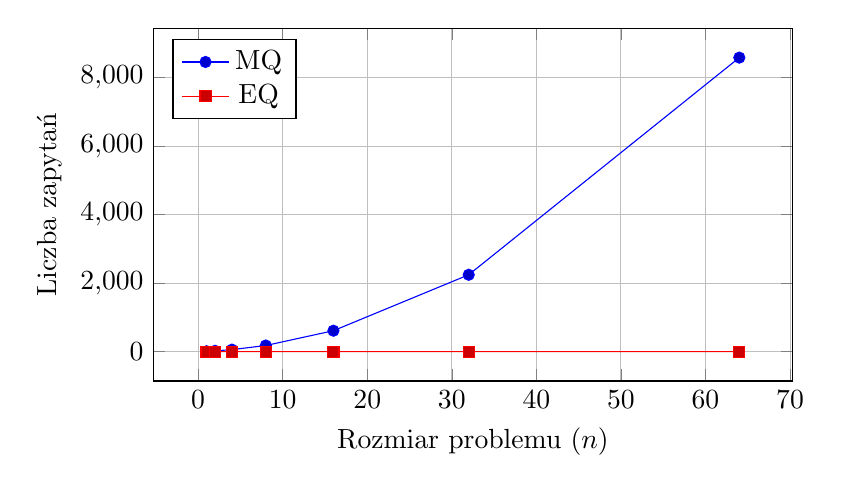
\begin{tikzpicture}
\begin{axis}[
    xlabel={Rozmiar problemu (\(n\))},
    ylabel={Liczba zapytań},
    legend pos=north west,
    grid=major,
    width=0.8\textwidth,
    height=0.5\textwidth
]

% MQ
\addplot coordinates {(1, 13) (2, 25) (4, 61) (8, 181) (16, 613) (32, 2245) (64, 8581)};
\addlegendentry{MQ}

% EQ
\addplot coordinates {(1, 2) (2, 3) (4, 3) (8, 3) (16, 3) (32, 3) (64, 3)};
\addlegendentry{EQ}

\end{axis}
\end{tikzpicture}
\caption{Zależność liczby zapytań EQ i MQ od rozmiaru problemu dla języka z sekcji \ref{sec:eksperyment1}.}
\label{fig:lstar_prefix_mq}
\end{figure}

\begin{table}[h]
\centering
\caption{Wyniki eksperymentu z sekcji \ref{sec:eksperyment2}.}
\label{tab:lstar_blocks}
\begin{tabular}{|c|c|c|c|}
\hline
Rozmiar problemu (\(n\)) & EQ & MQ & Rozmiar DFA \\ \hline
1                        & 3  & 24  & 4           \\ \hline
2                        & 4  & 54  & 6           \\ \hline
3                        & 5  & 104 & 8           \\ \hline
4                        & 6  & 180 & 10          \\ \hline
5                        & 7  & 288 & 12          \\ \hline
6                        & 8  & 434 & 14          \\ \hline
7                        & 9  & 624 & 16          \\ \hline
8                        & 10 & 864 & 18          \\ \hline
9                        & 11 & 1160 & 20         \\ \hline
\end{tabular}
\end{table}

\begin{figure}[h]
\centering
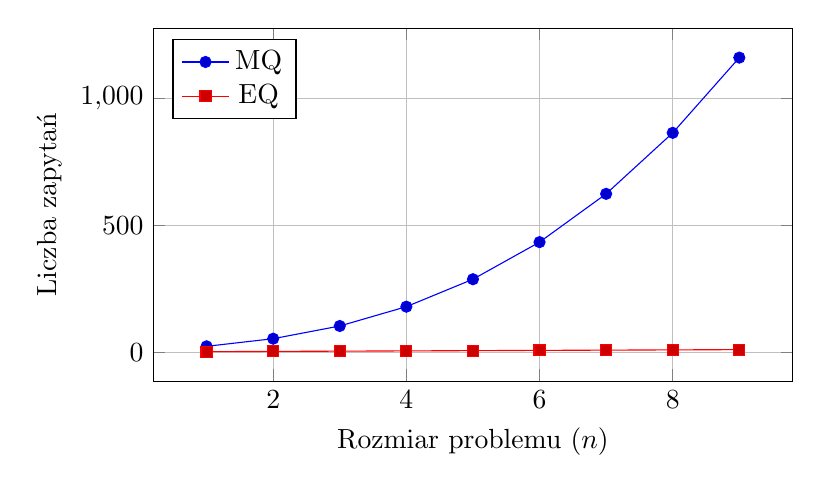
\begin{tikzpicture}
\begin{axis}[
    xlabel={Rozmiar problemu (\(n\))},
    ylabel={Liczba zapytań},
    legend pos=north west,
    grid=major,
    width=0.8\textwidth,
    height=0.5\textwidth
]

% MQ
\addplot coordinates {(1, 24) (2, 54) (3, 104) (4, 180) (5, 288) (6, 434) (7, 624) (8, 864) (9, 1160)};
\addlegendentry{MQ}

% EQ
\addplot coordinates {(1, 3) (2, 4) (3, 5) (4, 6) (5, 7) (6, 8) (7, 9) (8, 10) (9, 11)};
\addlegendentry{EQ}

\end{axis}
\end{tikzpicture}
\caption{Zależność liczby zapytań EQ i MQ od rozmiaru problemu dla języka z sekcji \ref{sec:eksperyment2}.}
\label{fig:lstar_blocks_mq}
\end{figure}


\section{Algorytm \textit{RPNI}}  
Eksperymenty dla algorytmu \textit{RPNI} miały na celu ocenę wpływu rozmiaru alfabetu na czas działania oraz strukturę wynikowego automatu. Testy przeprowadzono na językach z ciągami rozpoczynającymi się symbolem \( 0 \), po którym mogły występować dowolne symbole z danego alfabetu. Dane testowe przygotowano tak, aby liczba stanów w drzewie prefiksów (\textit{PTA}) była zbliżona dla różnych konfiguracji, co zapewniło porównywalność wyników.  

Tabela \ref{tab:rpni_results} przedstawia szczegóły wyników eksperymentu. Kolumna \textit{Rozmiar alfabetu (\(|\Sigma|\))} określa liczbę symboli w alfabecie testowego języka, a \textit{Liczba przykładów} podaje łączną liczbę danych wejściowych. Kolumny \textit{Stany PTA} i \textit{Stany DFA} przedstawiają odpowiednio liczbę stanów w drzewie prefiksów i wynikowym automacie deterministycznym (\textit{DFA}). Ostatnia kolumna, \textit{Czas [s]}, zawiera czas wykonania algorytmu.  

Wyniki pokazują, że czas działania algorytmu rośnie wraz z rozmiarem alfabetu (rys. \ref{fig:rpni_time}), choć dla alfabetu o rozmiarze 64 odnotowano krótszy czas niż dla 32. Może to wynikać ze specyfiki danych testowych lub procesu łączenia stanów. Liczba stanów w wynikowym automacie pozostaje niska, co świadczy o skuteczności algorytmu w uogólnianiu danych, jednak dla większych alfabetów (\(|\Sigma| = 16\) i \(|\Sigma| = 32\)) obserwuje się niewielki wzrost liczby stanów, co może sugerować trudności w uogólnianiu przypadków ze średnim rozmiarem alfabetu.  

Porównywalna liczba stanów w \textit{PTA} dla różnych rozmiarów alfabetów zapewniła rzetelność wyników, eliminując wpływ różnic w danych wejściowych. Algorytm \textit{RPNI} zachowuje wydajność przy różnych konfiguracjach parametrów, choć czas działania rośnie dla większych alfabetów.

\begin{table}[h]
\centering
\caption{Wyniki dla algorytmu \textit{RPNI}.}
\label{tab:rpni_results}
\begin{tabular}{|c|c|c|c|c|}
\hline
Rozmiar alfabetu (\(|\Sigma|\)) & Liczba przykładów & Stany PTA & Stany DFA & Czas [s] \\ \hline
2                               & 2807              & 5508.44   & 3         & 0.104656 \\ \hline
4                               & 1821              & 4993.48   & 3         & 0.166168 \\ \hline
8                               & 1673              & 5675.68   & 3         & 0.364098 \\ \hline
16                              & 1673              & 5307.78   & 3.58      & 0.644382 \\ \hline
32                              & 2257              & 5103.64   & 4.50      & 1.080040 \\ \hline
64                              & 4561              & 4756.92   & 3.06      & 0.883063 \\ \hline
\end{tabular}
\end{table}

\begin{figure}[h]
\centering
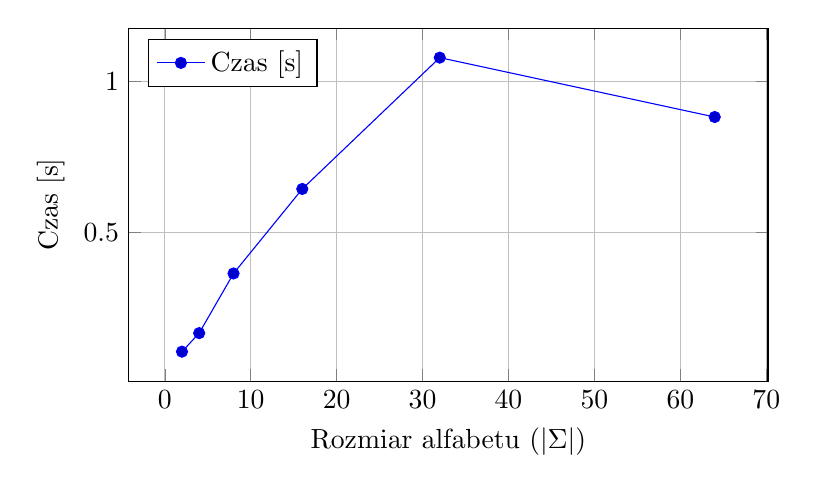
\begin{tikzpicture}
\begin{axis}[
    xlabel={Rozmiar alfabetu (\(|\Sigma|\))},
    ylabel={Czas [s]},
    legend pos=north west,
    grid=major,
    width=0.8\textwidth,
    height=0.5\textwidth
]
\addplot coordinates {(2, 0.104656) (4, 0.166168) (8, 0.364098) (16, 0.644382) (32, 1.08004) (64, 0.883063)};
\addlegendentry{Czas [s]}
\end{axis}
\end{tikzpicture}
\caption{Zależność czasu wykonania algorytmu RPNI od rozmiaru alfabetu.}
\label{fig:rpni_time}
\end{figure}


\section{Algorytm \textit{GIG}}  
Przeprowadzone eksperymenty dla algorytmu \textit{GIG} miały na celu zbadanie wpływu metody inicjalizacji populacji na jakość wynikowego automatu, liczbę generacji potrzebnych do uzyskania rozwiązania oraz dokładność klasyfikacji danych testowych.

Tabele \ref{tab:gig_one_a}, \ref{tab:gig_even_a} oraz \ref{tab:gig_even_a_or_b} prezentują wyniki uzyskane dla różnych metod inicjalizacji populacji. Kolumna \textit{Inicjalizacja populacji} określa zastosowany sposób inicjalizacji – \textit{warstwowa} oznacza podejście opisane w sekcji \ref{sec:gig-formalizacja}, natomiast \textit{losowa} generuje populację bez dodatkowych założeń. Kolumna \textit{Pokolenie} przedstawia średnią liczbę pokoleń potrzebnych do znalezienia rozwiązania. Kolumna \textit{Jakość} podaje skuteczność modelu jako procent poprawnych klasyfikacji. Kolumny \textit{TP} (True Positives) i \textit{TN} (True Negatives) wskazują odsetek poprawnych klasyfikacji przykładów pozytywnych i negatywnych, natomiast kolumny \textit{FP} (False Positives) i \textit{FN} (False Negatives) pokazują odsetek błędnych klasyfikacji.

Obie metody inicjalizacji populacji osiągnęły wysoką jakość klasyfikacji w każdym teście, lecz metoda losowa przyniosła lepsze rezultaty, skracając czas konwergencji średnio o $5.42$ pokolenia w teście trzecim (tabela \ref{tab:gig_even_a_or_b}). Sugeruje to, że losowość skuteczniej eksploruje przestrzeń rozwiązań, zwiększając prawdopodobieństwo znalezienia optymalnych modeli. 

Analiza wyników pokazuje, że metoda losowej inicjalizacji była bardziej efektywna dla złożonych języków, podczas gdy dla prostszych obie metody osiągały podobne rezultaty. Różnice w liczbie generacji okazały się niewielkie, co wskazuje, że wybór metody inicjalizacji miał większy wpływ na jakość wynikowych modeli niż na tempo konwergencji algorytmu.


\begin{table}[h]
\centering
\caption{Wyniki dla języka „Co najmniej jedno \( a \)” z sekcji \ref{sec:eksperyment4}.}
\label{tab:gig_one_a}
\begin{tabular}{|l|c|c|c|c|c|c|}
\hline
Inicjalizacja populacji & Pokolenie & Jakość & TP & TN & FP & FN \\ \hline
Inicjalizacja warstwowa & 94.64 & 0.944 & 0.889 & 1 & 0.111 & 0 \\ \hline
Inicjalizacja losowa    & 91.46 & 0.943 & 0.887 & 1 & 0.113 & 0 \\ \hline
\end{tabular}
\end{table}

\begin{table}[h]
\centering
\caption{Wyniki dla języka „Parzysta liczba \( a \)” z sekcji \ref{sec:eksperyment5}.}
\label{tab:gig_even_a}
\begin{tabular}{|l|c|c|c|c|c|c|}
\hline
Inicjalizacja populacji & Pokolenie & Jakość & TP & TN & FP & FN \\ \hline
Inicjalizacja warstwowa & 95.7  & 0.974 & 1 & 0.945 & 0 & 0.055 \\ \hline
Inicjalizacja losowa    & 96.44 & 0.987 & 1 & 0.973 & 0 & 0.028 \\ \hline
\end{tabular}
\end{table}

\begin{table}[h]
\centering
\caption{Wyniki dla języka „Parzysta liczba \( a \) lub \( b \)” z sekcji \ref{sec:eksperyment6}.}
\label{tab:gig_even_a_or_b}
\begin{tabular}{|l|c|c|c|c|c|c|}
\hline
Inicjalizacja populacji & Pokolenie & Jakość & TP & TN & FP & FN \\ \hline
Inicjalizacja warstwowa & 96.2  & 0.923 & 0.97  & 0.875 & 0.03  & 0.125 \\ \hline
Inicjalizacja losowa    & 90.78 & 0.968 & 0.988 & 0.948 & 0.013 & 0.053 \\ \hline
\end{tabular}
\end{table}


\section{Algorytm \textit{ALERGIA}}  
Badania nad algorytmem \textit{ALERGIA} skupiały się na ocenie jego odporności na szum w danych wejściowych. Analizowano jakość wynikowego modelu oraz liczbę stanów w wynikowym automacie w zależności od poziomu zakłóceń.

Podsumowanie wyników eksperymentu przedstawiono w tabeli \ref{tab:alergia_results}. Kolumna \textit{Procent szumu} określa poziom zakłóceń w danych wejściowych. Kolumna \textit{Jakość} podaje dokładność modelu jako odsetek poprawnych klasyfikacji wśród 10000 słów wygenerowanych z wynikowego automatu. Kolumna \textit{Stany automatu} wskazuje liczbę stanów w wynikowym automacie, co pozwala ocenić złożoność struktury modelu. Wszystkie wartości są uśrednione na podstawie powtórzeń testu.

Jak pokazują tabela \ref{tab:alergia_results} oraz wykresy \ref{fig:alergia_quality} i \ref{fig:alergia_states}, jakość modelu spada wraz ze wzrostem poziomu szumu w danych. Dla niskich zakłóceń (do 2\%) algorytm utrzymuje jakość powyżej 89\%, jednak przy 50\% szumu dokładność spada do około 74\%.  

Liczba stanów w wynikowym automacie wzrasta wraz z poziomem zakłóceń, co wskazuje na trudności w uogólnianiu danych przy większym szumie. Przy zakłóceniach do 10\% liczba stanów pozostaje stabilna, natomiast przy wyższych wartościach rośnie zauważalnie, odzwierciedlając większą złożoność modelu.

Wyniki eksperymentów pokazują, że algorytm \textit{ALERGIA} dobrze radzi sobie z niewielkimi zakłóceniami, zachowując wysoką jakość klasyfikacji i kompaktową strukturę automatu. W miarę wzrostu poziomu szumu jego zdolność do poprawnego odwzorowania języka stopniowo maleje, co objawia się zarówno spadkiem dokładności, jak i wzrostem liczby stanów automatu.

\begin{table}[h]
\centering
\caption{Wyniki dla algorytmu \textit{ALERGIA}.}
\label{tab:alergia_results}
\begin{tabular}{|c|c|c|}
\hline
Procent szumu & Jakość & Stany automatu \\ \hline
0             & 1.0000 & 2             \\ \hline
0.001         & 0.9941 & 2             \\ \hline
0.005         & 0.9734 & 2.14          \\ \hline
0.01          & 0.9527 & 2.56          \\ \hline
0.02          & 0.9280 & 3.30           \\ \hline
0.05          & 0.8921 & 3.92          \\ \hline
0.1           & 0.8985 & 4             \\ \hline
0.2           & 0.9100 & 4             \\ \hline
0.3           & 0.8664 & 4.32          \\ \hline
0.4           & 0.7998 & 4.98          \\ \hline
0.5           & 0.7412 & 5.36          \\ \hline
\end{tabular}
\end{table}

\begin{figure}[h]
\centering
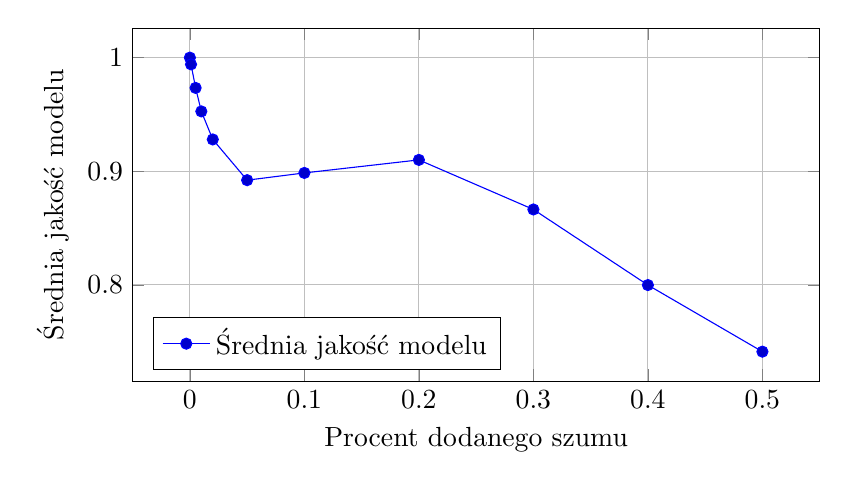
\begin{tikzpicture}
\begin{axis}[
    xlabel={Procent dodanego szumu},
    ylabel={Średnia jakość modelu},
    legend pos=south west,
    grid=major,
    width=0.85\textwidth,
    height=0.5\textwidth
]
\addplot coordinates {(0, 1.0) (0.001, 0.994074) (0.005, 0.97336) (0.01, 0.95268) (0.02, 0.927988) (0.05, 0.892144) (0.1, 0.898522) (0.2, 0.909984) (0.3, 0.866366) (0.4, 0.799828) (0.5, 0.741206)};
\addlegendentry{Średnia jakość modelu}
\end{axis}
\end{tikzpicture}
\caption{Zależność jakości modelu od poziomu szumu w danych.}
\label{fig:alergia_quality}
\end{figure}

\begin{figure}[h]
\centering
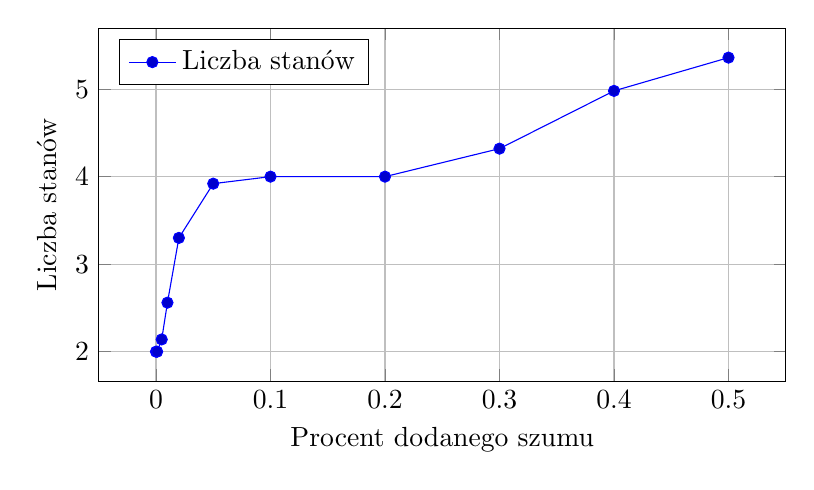
\begin{tikzpicture}
\begin{axis}[
    xlabel={Procent dodanego szumu},
    ylabel={Liczba stanów},
    legend pos=north west,
    grid=major,
    width=0.85\textwidth,
    height=0.5\textwidth
]
\addplot coordinates {(0, 2) (0.001, 2) (0.005, 2.14) (0.01, 2.56) (0.02, 3.3) (0.05, 3.92) (0.1, 4) (0.2, 4) (0.3, 4.32) (0.4, 4.98) (0.5, 5.36)};
\addlegendentry{Liczba stanów}
\end{axis}
\end{tikzpicture}
\caption{Zależność liczby stanów wynikowego automatu od poziomu szumu dodanego do danych.}
\label{fig:alergia_states}
\end{figure}


\section{Podsumowanie}  
Przeprowadzone eksperymenty pozwoliły na ocenę skuteczności i wydajności algorytmów \textit{L*}, \textit{RPNI}, \textit{GIG} oraz \textit{ALERGIA}. Algorytm \textit{L*} efektywnie generował minimalne automaty deterministyczne (\textit{DFA}), utrzymując niską liczbę zapytań o równoważność (\textit{EQ}), choć liczba zapytań o przynależność (\textit{MQ}) rosła wykładniczo wraz ze złożonością problemu, co czyni go odpowiednim w sytuacjach z dobrze zdefiniowanymi źródłami wiedzy. Algorytm \textit{RPNI} wyróżniał się prostotą, niską złożonością i wysoką wydajnością, co czyni go dobrym wyborem do szybkiego uogólniania danych, niezależnie od rozmiaru alfabetu. Algorytm \textit{GIG}, oparty na metodach ewolucyjnych, oferował elastyczność, lecz jego większa złożoność i czasochłonność nie zawsze przekładały się na lepsze wyniki w porównaniu z prostszymi metodami, a eksperymenty wykazały, że losowa inicjalizacja populacji częściej prowadziła do lepszych wyników niż inicjalizacja warstwowa. Algorytm \textit{ALERGIA} okazał się odporny na niewielkie zakłócenia, zachowując wysoką jakość klasyfikacji i kompaktową strukturę modelu, jednak jego skuteczność spadała przy większym poziomie szumu, co czyni go bardziej odpowiednim do danych probabilistycznych o umiarkowanym poziomie zakłóceń. Wybór algorytmu powinien być zatem dostosowany do specyfiki problemu – \textit{L*} sprawdza się tam, gdzie dostępna jest wyrocznia wysokiej jakości, \textit{RPNI} oferuje szybkość i prostotę, \textit{GIG} nadaje się do złożonych problemów optymalizacyjnych, a \textit{ALERGIA} jest przydatna w modelowaniu danych probabilistycznych.

    \chapter{Podsumowanie}
\label{cha:podsumowanie}  

Praca poświęcona była analizie zachowania i porównaniu czterech algorytmów indukcji gramatyk formalnych: \textit{RPNI}, \textit{L*}, \textit{ALERGIA} oraz \textit{GIG}. W jej ramach stworzono środowisko eksperymentalne, które umożliwiło ocenę tych metod pod kątem wydajności, dokładności oraz zdolności do uogólniania danych. Implementacja została zrealizowana w języku Python z wykorzystaniem bibliotek \textit{aalpy}, \textit{pygad}, \textit{numpy}, \textit{automata-lib} oraz \textit{pydot}, co pozwoliło na przeprowadzenie eksperymentów i wizualizację wyników.

Wykonana praca obejmuje opracowanie implementacji algorytmu \textit{GIG} z wykorzystaniem frameworku \textit{pygad}. W ramach tej implementacji autor zaadaptował operacje genetyczne, takie jak krzyżowanie i mutacja, opracował funkcje generujące populacje oraz zdefiniował funkcję przystosowania (\textit{fitness function}). Ponadto, zaimplementowano moduły uruchamiające eksperymenty, odpowiedzialne za konfigurację parametrów testowych i inicjalizację ich przebiegu. Oprócz tego autor stworzył funkcje wspomagające, takie jak mechanizmy generowania zbiorów danych, dodawania szumu do danych oraz obliczania jakości modeli. Kod został zaprojektowany w sposób umożliwiający jego rozszerzanie oraz ponowne wykorzystanie w przyszłych badaniach.  

Eksperymenty pozwoliły na ocenę skuteczności i wydajności badanych algorytmów. Algorytm \textit{L*} generował minimalne automaty deterministyczne (\textit{DFA}) przy niskiej liczbie zapytań o równoważność (\textit{EQ}), jednak liczba zapytań o przynależność (\textit{MQ}) rosła wykładniczo wraz ze złożonością problemu. Algorytm \textit{RPNI} wyróżniał się prostotą, niską złożonością i skutecznym uogólnianiem danych. Algorytm \textit{GIG}, choć oferował elastyczność dzięki zastosowaniu metod ewolucyjnych, nie zawsze przewyższał prostsze metody pod względem wyników, a losowa inicjalizacja populacji często prowadziła do lepszych rezultatów niż inicjalizacja warstwowa. Algorytm \textit{ALERGIA} wykazał odporność na niewielkie zakłócenia, jednak jego skuteczność malała wraz ze wzrostem poziomu szumu, co czyni go bardziej odpowiednim dla danych probabilistycznych o umiarkowanym poziomie zakłóceń.  

W trakcie realizacji pracy napotkano kilka wyzwań teoretycznych i praktycznych, które wymagały odpowiednich rozwiązań. Pierwszym problemem była ocena jakości modeli stochastycznych. Standardowe metryki, takie jak macierz pomyłek, nie mogły zostać zastosowane z uwagi na probabilistyczny charakter automatu. Rozwiązaniem było generowanie dużej liczby losowych zdań z automatu wynikowego i ich weryfikacja przez poprawny automat referencyjny. Pozwoliło to na przybliżoną ocenę jakości modeli.

Kolejnym wyzwaniem była sprawiedliwa ocena czasu działania algorytmu \textit{RPNI} w zależności od rozmiaru alfabetu. Czas działania algorytmu zależy od liczby stanów w akceptorze prefiksów (\textit{PTA}), która z kolei wynika z liczby i długości przykładów w danych wejściowych. Liczba stanów w \textit{PTA} jest trudna do przewidzenia i różni się w zależności od alfabetu, co utrudniało porównanie wyników. Problem rozwiązano poprzez ręczne dobieranie liczby przykładów, tak aby liczba stanów w \textit{PTA} była porównywalna dla różnych rozmiarów alfabetów.

Największym wyzwaniem w przypadku algorytmu \textit{GIG} było dobranie odpowiedniej funkcji przystosowania (\textit{fitness function}). Zbyt duży nacisk na minimalizację liczby stanów w automacie prowadził do utraty dokładności klasyfikacji, podczas gdy priorytetowanie poprawności klasyfikacji skutkowało generowaniem nadmiernie złożonych modeli. Rozwiązaniem okazało się empiryczne dostosowanie funkcji przystosowania, które uwzględniało zarówno minimalizację automatu, jak i jego dokładność. Funkcja wymagała jednak dopasowywania do specyfiki każdego przypadku, co wskazuje na potrzebę dalszych badań w tym obszarze.

Podsumowując, praca pozwoliła na stworzenie wszechstronnego środowiska testowego oraz przeprowadzenie szczegółowej analizy porównawczej algorytmów indukcji gramatyk formalnych. Wyniki eksperymentów wskazują na konieczność dopasowania wyboru algorytmu do specyfiki problemu i charakterystyki danych. Środowisko jest gotowe do dalszej rozbudowy, a przyszłe badania mogą objąć testy na danych rzeczywistych, optymalizację obecnych metod oraz analizę dodatkowych algorytmów.


\section{Dalsze kierunki rozwoju}
Możliwości dalszego rozwoju obejmują powtórzenie eksperymentów na bardziej złożonych lub rzeczywistych danych, co pozwoliłoby na dokładniejsze zbadanie praktycznych zastosowań algorytmów. Ponadto warto przeprowadzić dodatkowe analizy dla innych metod indukcji gramatyk formalnych, które nie zostały uwzględnione w tej pracy, w celu poszerzenia porównania i oceny ich skuteczności w różnych warunkach.

    
    % \appendix
    % \include{dodatek}
    % itd.
    
    \printbibliography

\end{document}
